\section{Příklad 2}
% Jako parametr zadejte skupinu (A-H)
\druhyZadani{B}

Pro potřeby výpočtu dle Théveninovy věty odpojíme zatěžovací rezistor, v našem případě označený $R_6$, a postupně vypočítáme napětí naprázdno.\\

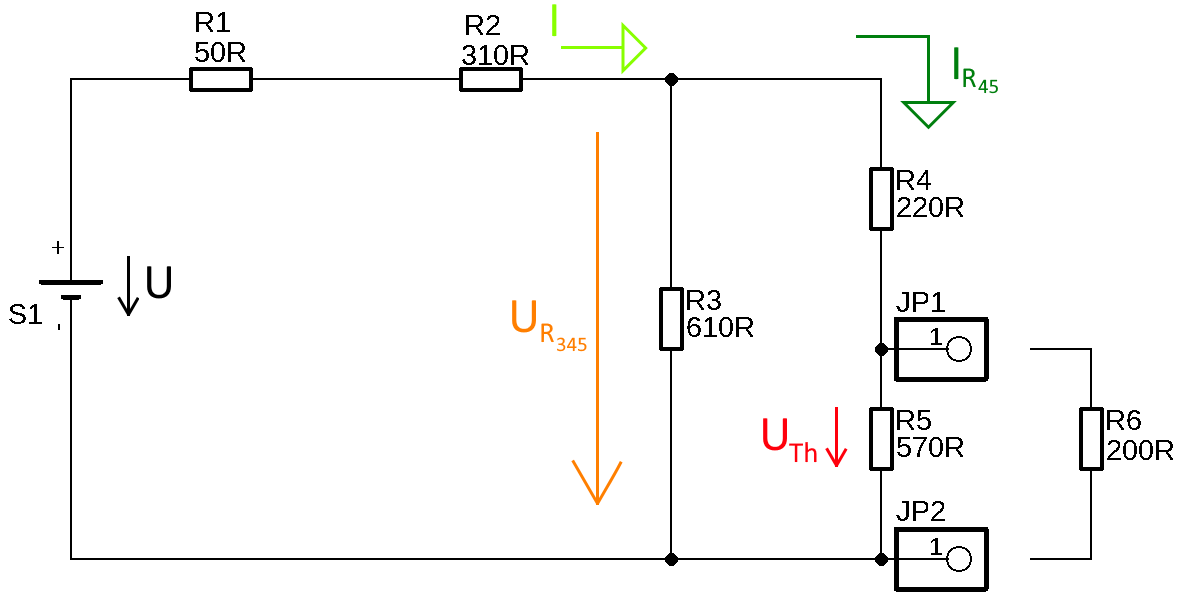
\includegraphics[totalheight=6cm]{fig/2_2.png}

Nejprve zjistíme odpor celé paralelní kombinace $R_3$, $R_4$, $R_5$ ($R_4$ a $R_5$ jsou sériově spojeny, můžeme je tedy sečíst):
{\large$$R_{45} = R_4 + R_5 = 220 + 570 = 790\:\Omega$$}
{\large$$R_{345} = \frac{R_3*R_{45}}{R_3 + R_{45}} = \frac{610*790}{610+790} = 344,2143\:\Omega$$}

Poté dle Ohmova zákona určíme napětí na paralelní kombinaci $R_{345}$:
{\large$$U_{R_{345}} = I * R_{345} = \frac{U}{R_1+R_2+R_{345}} * R_{345} = \frac{100}{50+310+344,2143} * 344,2143 = 48,8792\:V$$}

Napětí naprázdno podle Théveninovy věty (zde na rezistoru $R_5$, ke kterému se paralelně připojuje zátěž) zjistíme pomocí Ohmova zákona:
{\large$$U_{Th} = I_{R_{45}}*R_5 = \frac{U_{R345}}{R_{45}}*R_5 = \frac{48,8792}{790}*570 = 35,2673\:V$$}

\newpage
Poté vyzkratujeme napájecí zdroj a vypočítáme ekvivalentní předřadný vnitřní odpor $R_i$ zdroje podle Théveninovy věty: \\

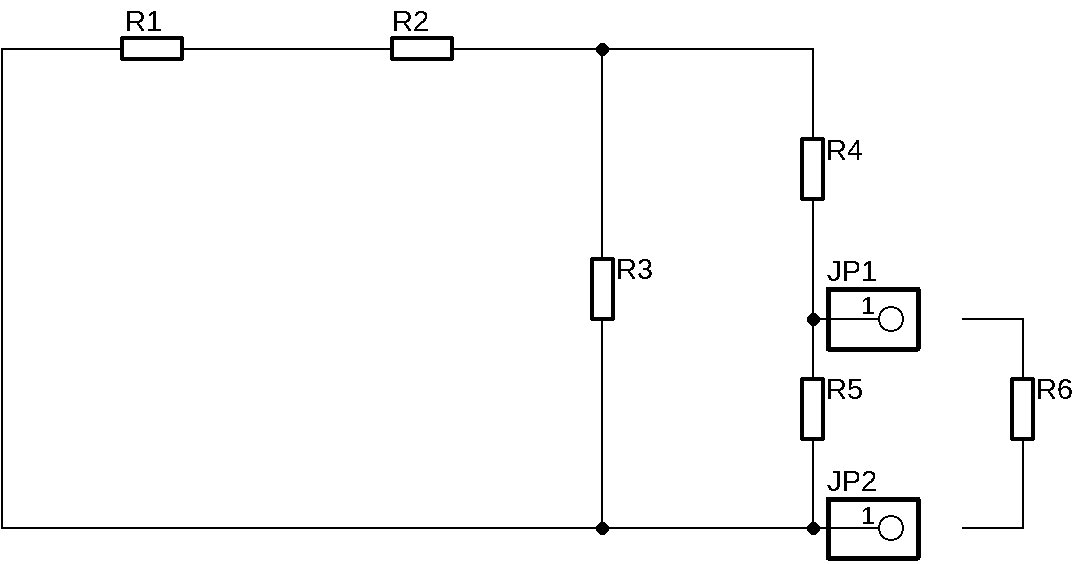
\includegraphics[totalheight=6cm]{fig/2_3.png}

Nejprve musíme provést ekvivalentní úpravu trojúhelníkového zapojení rezistorů na hvězdu:
{\large$$R_A = \frac{R_4*R_5}{R_3+R_4+R_5} = \frac{220*570}{610+220+570} = 89,5714\:\Omega$$}
{\large$$R_B = \frac{R_3*R_5}{R_3+R_4+R_5} = \frac{610*570}{610+220+570} = 248,3571\:\Omega$$}
{\large$$R_C = \frac{R_3*R_4}{R_3+R_4+R_5} = \frac{610*220}{610+220+570} = 95,8571\:\Omega$$}

Vznikne nám následující obvod: \\

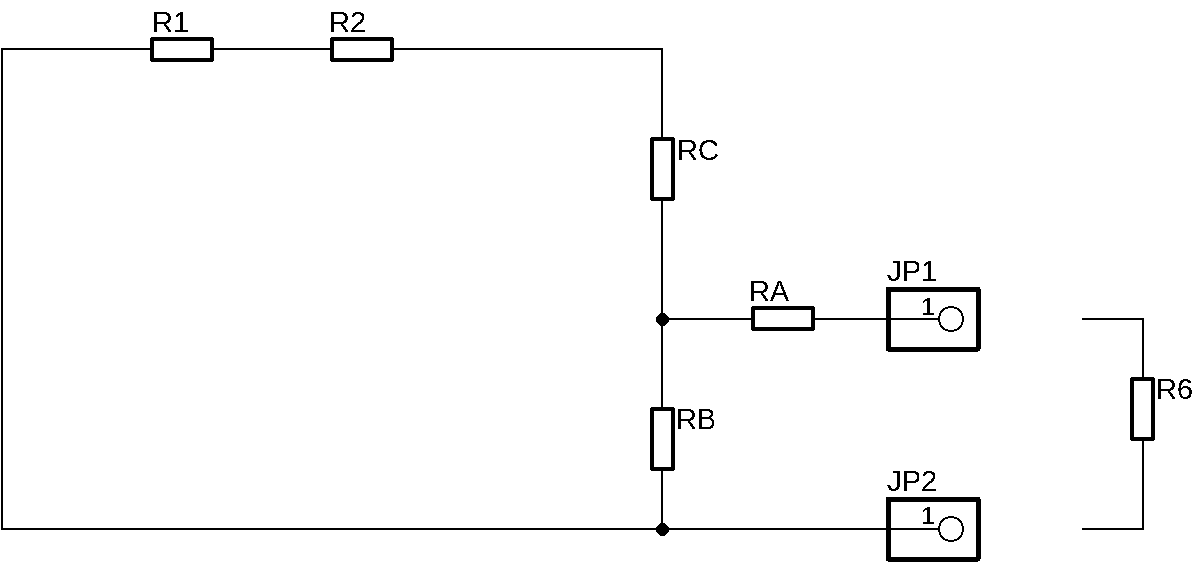
\includegraphics[totalheight=6cm]{fig/2_4.png}

\newpage
Vidíme, že rezistory $R_B$, $R_C$, $R_1$ a $R_2$ tvoří serioparalelní kombinaci.

Seriově zapojené rezistory sečteme a vypočítáme odpor paralelní kombinace:
{\large$$R_{12C} = R_1 + R_2 + R_C = 50 + 310 + 95,8571 = 455,8571\:\Omega$$}
{\large$$R_p = \frac{R_{12C} * R_B}{R_{12C}+R_B} = \frac{455,8571*248,3571}{455,8571+248,3571} = 160,7683\:\Omega$$}

Takto vypadá mezikrok výše: \\

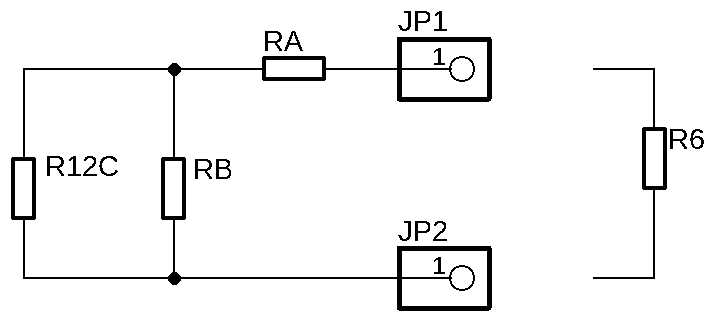
\includegraphics[totalheight=4cm]{fig/2_5.png}

Na závěr sečteme nově vzniklé seriové zapojení rezistorů, čímž konečně získáme velikost odporu $R_i$:
{\large$$R_i = R_A + R_p = 89,5714+160,7683 = 250,3397\:\Omega$$}

Výsledkem je toto zjednodušení: \\

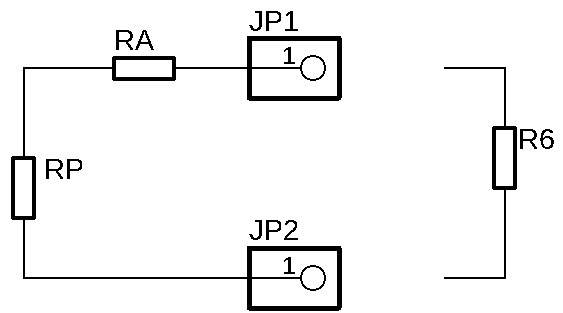
\includegraphics[totalheight=4cm]{fig/2_6.png}

Nyní k ekvivalentnímu ideálnímu zdroji s napětím $U_{Th}$ a jeho vnitřnímu odporu $R_i$ můžeme připojit zatěžovací rezistor $R_6$: \\

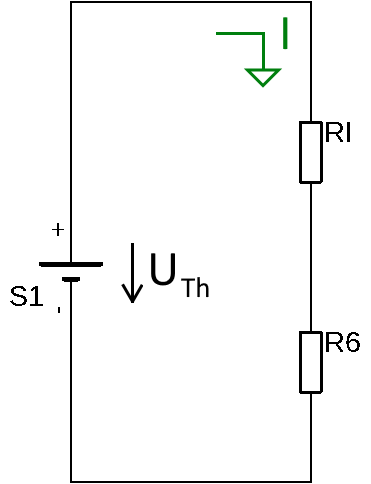
\includegraphics[totalheight=5cm]{fig/2_7.png} 

\newpage
Proud rezistorem $R_6$ ($I = I_{R6}$) zjistíme podle Ohmova zákona:
{\large$$I =\frac{U_{Th}}{R_i+R_6} = \frac{35,2673}{250,3397+200} = 78,3127\:mA\approx0,07831\:A$$}

Z proudu a odporu zátěže zjistíme podle Ohmova zákona napětí na zátěži:
{\large$$U_{R6} = I*R_6 = 78,3127 * 10^{-3} * 200 = 15,6625\:V$$}